\documentclass{standalone}

\usepackage{tikz}

\begin{document}
	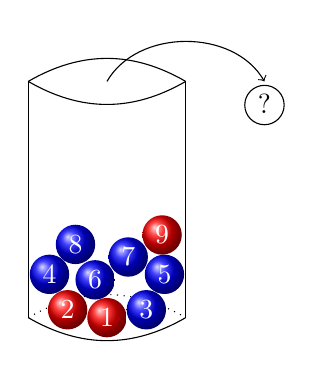
\begin{tikzpicture}
		\draw (0,0) -- (0,-3);
		\draw (2,0) -- (2,-3);
		\draw (0,-3) to [bend right] (2,-3);
		\draw[dotted] (0,-3) to [bend left] (2,-3);
		\draw (0,0) to [bend right] (2,0);
		\draw (0,0) to [bend left] (2,0);
		
		\begin{scriptsize}
		\shade [ball color=red] (1,-3) circle (0.25cm);
		\shade [ball color=red] (0.5,-2.9) circle (0.25cm);
		\shade [ball color=blue] (1.5,-2.9) circle (0.25cm);
		\shade [ball color=blue] (0.27,-2.45) circle (0.25cm);
		\shade [ball color=blue] (1.73,-2.45) circle (0.25cm);
		\shade [ball color=blue] (0.85,-2.52) circle (0.25cm);
		\shade [ball color=blue] (1.27,-2.23) circle (0.25cm);
		\shade [ball color=blue] (0.6,-2.07) circle (0.25cm);
		\shade [ball color=red] (1.7,-1.95) circle (0.25cm);
		\end{scriptsize}
		\node[white] at (1,-3) (1) {1};
		\node[white] at (0.5,-2.9) (2) {2};
		\node[white] at (1.5,-2.9) (3) {3};
		\node[white] at (0.27,-2.45) (4) {4};
		\node[white] at (1.73,-2.45) (5) {5};
		\node[white] at (0.85,-2.52) (6) {6};
		\node[white] at (1.27,-2.23) (7) {7};
		\node[white] at (0.6,-2.07) (8) {8};
		\node[white] at (1.7,-1.95) (9) {9};
		
		\draw[->] (1,0) to [bend left=60] (3,0);
		\draw (3,-0.3) circle (0.25cm);
		\node at (3,-0.29) (a) {?};
	\end{tikzpicture}
\end{document}